\chapter{寻找改进机会} % Introduction chapter suppressed from the table of contents

如果贵公司计划在8个月后进行质量改进（如ISO或CMMI），但当前缺少必要的过程文件和指导方针，该如何应对？\\
三年前，我们确实遇到了类似的情况。幸好咨询公司告诉我们不必担心，他们根据其他已经通过评估的公司整理了一整套完整的流程、模板和指南，确保能够满足评估要求。评估前，我们安排项目组根据过程和模板准备了相关的项目文档，一个月后顺利通过评估。''\\
请问你们现在还继续使用吗？\\
评估通过后，团队便恢复了原有的工作方式，不再使用咨询公司提供的那套文档了。但我在电脑上还是保留了备份。''\\
从以上对话中，我们看仅仅要求团队使用第三方的最佳实践，常常难以落地，对流程和质量的提升也没有实际帮助。那么，为什么团队会抗拒这些原本非常有价值的模板和指南呢？背后的原因是什么？\\

\hypertarget{ux7834ux51b0---ux53d8ux9769---ux7a33ux5b9a}{%
\subsection{破冰 - 变革 -
稳定}\label{ux7834ux51b0---ux53d8ux9769---ux7a33ux5b9a}}

一些美国企业，如通用和福特，相信科学管理。例如，老福特曾邀请
Taylor先生优化汽车生产线，但他的优化主要集中在工程层面，忽视了一线员工的参与，这导致许多一线工人抵触由``工程师''用科学方法设计的最佳方案。\\
为什么过程改进的落地如此困难重重？又为何遭到工人的反对？要解答这些问题，需要先了解人类的心理。\\
心理学教授Lewin发现，任何过程改进，例如费城Weisbord先生的自主团队改革，都需经过以下三个阶段：\\
第一、破冰（Unfreezing）阶段，通过提供新的信息和数据，减少团队的反对声音，动摇原有习惯，促进``破冰''。\\
第二、变革（Moving）阶段，促使团队改变态度、价值观、架构和行为等。\\
第三、固化（Refreezing）阶段，在取得成效后，持续维护改进成果，避免回归旧习。

增量过程改进 如下图所示，显示每轮都有提升。


%\href{文件:图9-1.jpg}{500px}

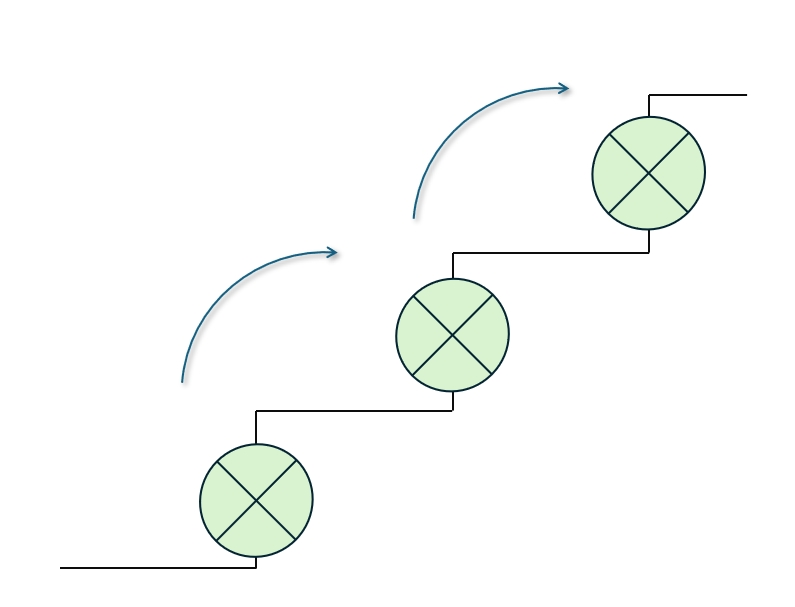
\includegraphics[width=10cm]{图9-1.jpg}

图9-1

Dr.
Lewin在分析二战粮食分配实验（见附件）时发现：``必须让人们参与分析和讨论，才能激发他们采取行动的动力。We
are likely to modify our own behavior when we participate in problem
analysis and solution, and likely to carry out decisions we have helped
make.''\\
美国弗吉尼亚州的Harwood工厂也做了一个实验，允许团队自主安排工作以应对季节性市场需求的变化，结果表明让团队自主策划效果最佳（详见本文附件``睡衣工厂试验''）。\\
这两个实验都验证了集体讨论与自主管理确实能够提升团队的生产率，同时也印证了实验前的观察：不同工人有各自不同的工作方式。\\

\hypertarget{ux81eaux5df1ux627eux7b54ux6848}{%
\subsubsection{自己找答案}\label{ux81eaux5df1ux627eux7b54ux6848}}

丰田强调``自己找答案''和``生产产品就是培养人''。因此，即便过程改进小组知道如何有效解决一线员工问题的方法，他们也不会直接提供答案，而是鼓励员工自主思考寻找解决方案。\\
为什么呢？\\
因为丰田管理层的信念就是：人的智慧没有尽头。过多干预不仅会阻碍员工发挥无限潜能为公司增值，还容易传递``员工必须服从指挥''的信息，助长企业内的``大王''文化，类似于前述谷歌的``河马''文化。\\
鼓励员工通过动脑思考和总结经验教训，是培养人才的必经之路。\\
从丰田的案例和Dr.
Lewin的实验可以看出，群体参与的重要性。让员工有机会参与或影响决策，他们就有动力推动改进。反之，如果只是要求员工遵循专家的``最佳方案''，则难以激发他们主动进行实验和分析数据。下面另一个实验可以让我们更理解：

\framebox{%
\begin{minipage}[t]{0.97\columnwidth}\raggedright
自己做实验，分析数据
有家工厂，很多主管不愿意雇佣30岁以上的女性操作工，认为她们的生产效率不如年轻女工。若我们作为顾问，直接提供数据证据，能改变这种看法吗？不太可能。所以顾问只能鼓励他们自己进行实验，证明那些
30岁以上女工的生产率确实比年轻女工的要低。所以顾问只能鼓励他们自己进行实验，证明那些
30岁以上女工的生产率确实比年轻女工的要低。从此，这些主管不再拒绝聘用年长的女工了。但那些没有参与实验的团队依旧不愿意改变他们的观念。

\strut
\end{minipage}}

\hypertarget{ux6210ux529fux8981ux7d20}{%
\subsection{成功要素}\label{ux6210ux529fux8981ux7d20}}

从此，这些主管不再拒绝聘用年长的女工了。但那些没有参与实验的团队依旧不愿意改变他们的观念。以下是他的经验分享：\\
在为企业做访谈和诊断时，一般的顾问仅关注企业遇到了什么问题、有什么困难及其解决方法？而更为有效的是跳出这个圈子，从更高的视角去思考这家公司有哪些改进的潜力？公司内部是否有能够持续推进这种改革的人？是否存在一些可以吸引全员参与的改革方向？随着环境快速变化，顾问的角色不应再局限于帮助客户解决技术问题或提供诊断方案，而是转向挖掘员工的潜力，让他们主动思考并解决自身遇到的问题。只有这样，才真正对企业有价值。''\\
他提出了三个成功的关键因素：

\hypertarget{leadership-commitment-ux9886ux5bfcux652fux6301}{%
\subsubsection{Leadership commitment
领导支持}\label{leadership-commitment-ux9886ux5bfcux652fux6301}}

有没有领导的支持？\\
我接触过很多公司，如果高层难以联系或并不关心质量问题，甚至认为可以委托他人处理，推进就会变得困难。常见的情况是领导本身业务出身，也不关注软件工程，认为软件开发并不复杂，市场和销售才是重点。或者，领导只是口头上支持，实际上没有定期监控改进的进展，对培训也不太关注，最终很难取得实质性效果。

\hypertarget{ux5546ux673a-good-business-opportunity}{%
\subsubsection{商机 Good Business
opportunity}\label{ux5546ux673a-good-business-opportunity}}

公司有没有一些持久的商机？\\
当前软件工程的竞争激烈。如果公司没有持久的方案、产品或专注的业务方向，而是靠客户关系做些定制开发的项目，就很难投入资源进行提升。

\hypertarget{ux5458ux5de5ux52a8ux529b-energized-people}{%
\subsubsection{员工动力 Energized
people}\label{ux5458ux5de5ux52a8ux529b-energized-people}}

公司里面有没有中层愿意投入时间，真心推动改革？\\
如果谷歌没有Smart
Creatives这样的员工，就不会有如此多的谷歌创新产品。如果员工都是负面的心态，推动改进将困难重重。\\
关于第一点领导支持，前面已经分享了如何用高层的语言（金钱、成本）吸引他对改进感兴趣，然后估计能节省多少，并正式立项。\\
有了这些基础，便可以开始质量改进之旅。

\hypertarget{aux516cux53f8ux8fc7ux7a0bux6539ux8fdbux4e4bux65c5}{%
\subsection{A公司过程改进之旅}\label{aux516cux53f8ux8fc7ux7a0bux6539ux8fdbux4e4bux65c5}}

今年4月初，我首次拜访A公司高层，听他们过程改进需求。\\
COO万先生最后一位到，看来50多岁，中等身材，身穿有公司标志的长袖外套，工程师打扮，留了一点胡子，精神饱满。他非常忙，只能空出半小时。\\
我们甲乙双方各2位，开始围着小圆桌交流。\\
COO谦虚地说：``我没有软件开发项目经验，一直都是管理基础建设项目。我之前见过任正非，当时公司帮华为在香港建设数据中心。''\\
万先生是高层团队成员之一，与集团主席、副主席、总经理、财务总监等共7人组成高层团队。\\
我简单介绍了CMMI是用于衡量公司的过程成熟度模型,软件开发供应商一直质量水平差异很大。接着说：``软件项目不同于硬件项目，交付后会根据需求不断变动。如果开发期间不注重质量，又缺乏评审和测试，产品会有许多缺陷。由于软件本身设计不佳，最终引发大量返工工作。就像埋下了大量地雷，后面需要还债，这叫`技术债务'（Technical
Debt）。编码人员为了省时间，只顾写代码，缺乏文档，其他人难以看懂，几周后甚至自己也看不懂，导致后续还债更加困难。所以虽然小学生都可以写程序，但不一定能写出灵活、高质量的程序。''\\
看到COO深有感触，他望着旁边的老王（部门经理）说：``你说得对，我们现在也正在还债。''\\
接着，他介绍了集团的组织架构：主要有4个业务部，最大的是工程部，承接大厦的电机工程，例如电梯、空调、自动化等；专门做政府软件项目的部门叫科技部（约80名员工），虽然业务部门，如工程部也逐步拓展了软件服务部分，但占总体业务收入不到5\%。\\
COO预计咨询顾问可能怀疑他们做过程改进的决心，便解释说之前已经跟其他董事会成员说过：``虽然现在软件开发占公司业务量不多，但包括软件部分的项目（如办公楼的自动化）越来越多，并有不断上升趋势，这将是我们未来核心竞争力的重要部分。所以必须预先练好内功，才有能力在未来承接更多的软件相关项目。''\\
他再强调公司不仅仅是为了拿到CMMI证书，更重要是希望改进我们软件开发过程。\\
项目启动后，从4月底到5月初为他们的6位评估组成员，做了8天培训。\\
很佩服万总的魄力和支持，在第一天培训开始前，他特意找了公司总经理来培训现场给各学员说话，打气。虽然万总每天都非常忙，但他还是尽量抽一些时间来听课。\\
但因为COO万总确实太忙了。我们解释了如果没有一位有经验的人领导改进组，后面难以推进，他便联系老刘，请他担任组长。\\
老刘进A公司已经16年了，年龄与他接近，是整个集团培训中心的负责人。\\
6月底，公司安排了午饭期间，我与COO安排的过程改进组长刘先生在培训中心旁边的Ibis酒店首次见面。刘先生问：``请问过程改进小组是做什么的？虽然我一直负责工程项目和质量，但对软件开发并不熟悉，这样能胜任吗？''\\
``非常欢迎你来当组长，我们非常需要像你这样有经验的管理层来推动过程改进。你不用担心不熟悉软件开发，我已经和相关的项目经理、评估组成员、QA等进行了几天的深入培训，他们很清楚需要改进和欠缺的地方。组长的主要职责是协助这些改进组，一方面为他们争取所需要的资源，另一方面向高层汇报，让他们了解改进的价值并获得支持。''\\
老刘问：``软件工程的质量问题与一般工程项目有什么不一样吗？''\\
我解释：``现在我们周围的日常产品大多都包含软件，因为软件比硬件灵活，功能更新也容易。以前在硬件上做变动很困难，而软件则不同。正因为软件容易更新，我们在写程序时必须确保代码易于增加或删除功能。如果程序写得不好，任何改变都可能导致整个程序的大幅改动或重写，这就是所谓的`技术债务'。''\\
老刘说：``这跟我们做工程项目很不一样，很多项目在交付前，业主还是会提很多修改。比如某些管道怎么走，因为这些修改不影响建筑结构，所以我们还是会按要求修改。''\\
旁边的小李（A公司项目经理）补充道：``我听说去年某项目团队，因为前期过程，如单元测试、集成测试等都没做好，也缺少报告与文档，最终导致客户在验收时拒收。团队尽力补救，但那些阶段已经过去，无法弥补。管理层为了避免项目烂尾，影响声誉，承诺把整个项目从头再做。客户因为有了经验教训，特意找了第三方公司监督项目的过程。所以我们非常同意前期如果不注意质量，后期就要还债。''\\
后面边吃边聊中，了解到老刘一直保持运动。年轻时他喜欢打壁球，但因为壁球需要前后快速移动，容易伤到膝盖，所以年纪大了改为跑步。他每天6点起床，7点前跑步。如果周末不用上班，他早上会跑步大约一小时。\\
过程改进小组正式成立，并由老刘担任组长，负责监督每月的小组会议，尽管会议有纪要和待办事项，但3个月过去了，进展并不明显。

\begin{description}
\tightlist
\item[]
= = = =
\end{description}

9月底，过程改进小组开第二次会议，参与的人数比上次多，有四、五位组长参加，大家积极参与讨论，组长熟悉了整个过程改进的监控。例如用了2小时讨论配置管理的问题和改进后，组长与大家确认是否所有要改进的点都讨论完毕，并把具体的改进工作分配到对应的人，大家决议用2周一轮冲刺的方式来评估进展。\\
参与的人也主动提出要做什么改进的工作，整个气氛比上次好多了，但还是没有形成一个具体任务工作分解（WBS）的计划。\\
因为过程改进如果没有分到任务的计划，很容易会延误，后面就没有冲劲。但外部顾问暂时难以直接把问题说出来，唯有静观其变，原先的总体计划是4月份启动，10月份做预评估，但到了9月份大家发现进展缓慢，所以调整计划把预评估延到2月份，也计划在11月初在香港，安排了我到现场做一天补充培训。

\hypertarget{ux5341ux6708ux4efdux4e00ux5929ux57f9ux8bad}{%
\subsubsection{11月份一天培训}\label{ux5341ux6708ux4efdux4e00ux5929ux57f9ux8bad}}

早上5个部门的领导，加上万总、老刘都参加，除了2位，其他5位都是首次见面。我先跟他们说因前面评审和测试不足，大部分缺陷都在后面测试时才被发现处理，导致大量可以避免的返工。也介绍了``技术负债''。
我继续解释该如何选择------第一个改进项目的方向很重要。因为最终必须为公司省钱，管理层才会继续支持，所以必须能节省成本或工作量。也必须可度量。我接着解释为什么建议应针对如何能尽早发现并解决缺陷，避免后面大量返工。这样便能不仅仅是质量最优（留给客户的缺陷数最少），也能降低总工作量。\\
各领导都纷纷表示赞同。\\
午饭后，大家开始做互动练习，但大部分领导没有参加，主要是项目经理和评估组成员。在培训结束前最后一小时，邀请万总和老刘来现场，跟5个项目组长说好要星期一提交改进计划，但过了期限没有任何回应，过了3天万总亲自发邮件催促，再过2天才有其中一组回邮件发计划，但已经晚了一周，再过几天另一组也发了计划，其他3组一直没有反应。\\

这两组计划。其中一组只提交了进度表；另一组误以为只需要写一下过程文件，满足两个月后的评估需求。所以没有一个合格的计划。\\
我立马反馈给高层管理说明改进计划应包括什么内容，例如必须要有量化目标，明确团队成员和改进的里程碑和相关的培训和辅导等。\\

\hypertarget{ux56deux987eux8fdbux5c55ux7f13ux6162ux7684ux539fux56e0}{%
\subsection{回顾进展缓慢的原因}\label{ux56deux987eux8fdbux5c55ux7f13ux6162ux7684ux539fux56e0}}

除了高层支持和人员参与外，也需要有工具配合。例如：项目管理工具。\\
如果已经有明确量化改进目标，也有所需要的资源，包括人员和工具，我们还需要有一张地图，在敏捷开发过程改进中，可以参考Scrum、XP极限编程、CMMI等。

%\href{文件:三个圈圈20241028.jpg}{600px}

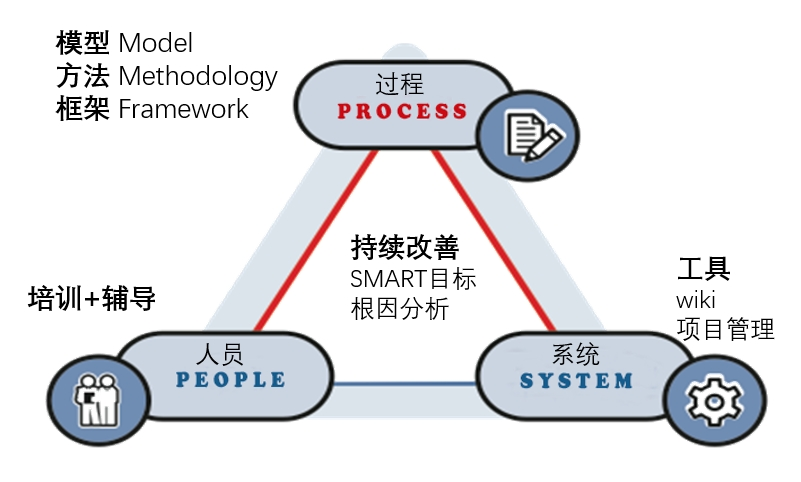
\includegraphics[width=10cm]{三个圈圈20241028.jpg}

图9-2

例如如果依据CMMI里针对估算、策划和监控的实践要求，便能列出项目管理工具需要以下项目管理工具应具备的基本功能：\\
*有日期和可交付成果的WBS管理\\
*个人更新工时表，更新任务实际开始/完成日期\\
*只有经过同行评审，任务才能100\%完成\\
*实时项目状态：例如红黄绿、挣值分析（进度变量\%，成本变量\%）\\
A公司的过程改进在哪些地方出了问题？\\
一直没有把过程改进当成一个项目来管理，进展缓慢，但因没有项目实际与计划对比的监控，大家都不知道确实延误了多少。（只知道现在是有延误）\\
*虽然COO从头一直尽力推动
，但部门级领导参与不多。因为软件开发人员都忙于做项目，从5月份开始一直都是由共6位从部门安排的代表参加。例如很多部门经理只是11月初来参加了上午半天培训。下午到做互动练习是他们的手下做项目的工程师来参加，到了最后要制定行动计划和目标时，部门经理都不在\\
*虽然在5月份做了共8天培训，但一直没有改进计划，导致培训内容与实际改进行动难以对应\\
*虽然做了五天专题培训，包括测试、功能点估算、需求、项目策划与监控、配置管理等，但因为没有立马在项目使用，没有效果\\
综上所述，目前的状况不是特别意外，虽然大部分参加培训的成员开始时都相当积极，但碍于他们的领导缺乏投入，导致没有进展。因为大部分团队，不论组长或者组员都没有经历过过程改进，所以开始时会走很多弯路。\\
虽然培训很重要，但最困难是改变人的习惯，培训本身不能改变团队的思路和做事习惯，如果公司不把过程改进作为项目来管理，投入资源并定期监控，培训不会为公司带来任何价值，员工也没有动力参加。

\hypertarget{ux5982ux4f55ux80fdux52a0ux5febux7834ux51b0}{%
\subsection{如何能加快破冰}\label{ux5982ux4f55ux80fdux52a0ux5febux7834ux51b0}}

传统咨询辅导的方式：先诊断发现差距，针对不足做培训，在某些项目试点，然后推广，再评审。前后会跨越好几个月。以A公司为例，除了要解决管理层参与、人员有充分时间投入与工具等基础问题外，如想改进能尽早有效果，考虑所有干系人聚在一起，做2天工作坊，大家针对改进主题讨论，出目标与计划。\\
针对以上传统做法的不足，如果把所有干系人聚在一起，做2天工作坊，一起回顾过去，放眼未来，制定具体量化目标和行动计划，便能让``所有员工参与改进整个系统''便能改善各种沟通不畅的问题。把本来需要几周时间沟通，压缩到2天。

%\href{文件:图2-2.jpg}{600px}

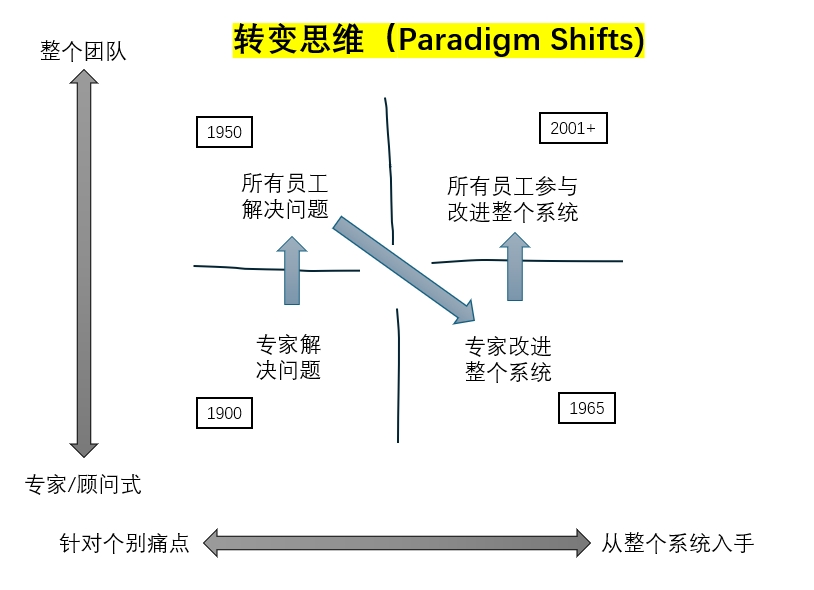
\includegraphics[width=10cm]{图2-2.jpg}

图9-3

（参考M. Weisbord,Productive Workplaces Revisited）

\framebox{%
\begin{minipage}[t]{0.97\columnwidth}\raggedright
过程重组\\
因为IBM的机器很昂贵，大部分客户需要安排分期付款。针对这客户需求，IBM公司成立子公司专门提供贷款服务。
整个过程共5个步骤：初步审核、查看公司的财政背景、专人制定的贷款的利率、法务看合同条款、文员把合同打印好交给销售人员，平均需要六个工作日，但有时候可以长达两周。在这段时间，客户可能会找到更好的贷款渠道，或者竞争对手导致客户改变主意，所以一线销售人员一直觉得时间太长，并会不停催促。\\ 为了解决这个问题，2位IBM高级经理专门头脑风暴研究是否可以缩短整个过程。他们先实验，把这5个部门的工作集中一起做，发现总共只需要90分钟（一个半小时）。中间大部分时间浪费在部门之间信息交流、等待。
他们发现开始提供贷款服务时，认为每一个步骤都需要专业人事处理。但他们发现除了少数特别情况，大部分交易都可以标准化处理。例如把各种情况列出来，并预先先定好对应的价位和利率，和标准合同模板等等，都预先记录在电脑中。有了这些信息化支持，这种改善做完以后，这些本来由专家负责的工作便可合成由一个人负责。\\ 结果把本来六七天的流程减到4小时。\\ 这类改善并非渐进式，而是改革式，从基础总体看问题，因为不能仅仅是按现在的流程做优化，必须从整个流程从头到尾看才可以取得效果。
\strut
\end{minipage}}

``我们开发人员天天加班，尽力满足需求，但产品经理提的需求都写的很模糊，又经常改变，后面系统测试发现很多缺陷，不能但怪罪我们开发人员。''\\
``我们测试人员要做好测试真是很困难，前面开发人员没有做好自测，写完代码就扔给我们测试，肯定会发现很多缺陷，但项目经理又要求我们赶上在发版日前完成，真不晓得应怎样做。''\\
大家都可能听过以上的声音。跟上面IBM的案例一样，不能单靠某部门去改善总体效果，需要各部门都参与，才可以提升，最终达到公司的目标。

若要所有员工参与，有效改进整个系统，要注意以下4条原则：

\hypertarget{ux8ba9ux56e2ux961fux81eaux5df1ux5bfbux627eux6539ux8fdbux65b9ux6848}{%
\subsubsection{让团队自己寻找改进方案}\label{ux8ba9ux56e2ux961fux81eaux5df1ux5bfbux627eux6539ux8fdbux65b9ux6848}}

上面粮食分配实验也验证了团队只有兴趣执行自己集体讨论的分析结果，而非听从``专家''意见。所以必须让大家参与、动脑筋，才有动力采取行动。\\
让每位团队成员都有充分机会表达意见，集思广益，得出更好的纠正措施。

\hypertarget{ux6574ux4e2aux56e2ux961fux6240ux6709ux76f8ux5173ux5e72ux7cfbux4ebaux53c2ux4e0e}{%
\subsubsection{整个团队（所有相关干系人）参与}\label{ux6574ux4e2aux56e2ux961fux6240ux6709ux76f8ux5173ux5e72ux7cfbux4ebaux53c2ux4e0e}}

整个团队分析全局问题。例如如果只是从测试人员的角度，他可能以为缺陷都是来自开发；需求分析人员（或产品经理）会觉得自己做得很好，因需求评审里没有什么问题被发现。但如果团队所有成员聚在一起（包括项目经理、需求、设计、编码、测试），让团队所有岗位一起分析，才可以全局看问题，才可能发现不少问题是因为需求没有明确，导致后面做出来的功能并不是客户要的。后面可扩大参与回顾的干系人，例如客户代表，可以更全面分析。\\

\hypertarget{ux770bux5168ux5c40ux5bfbux627eux5927ux5bb6ux7684ux5171ux540cux70b9}{%
\subsubsection{看全局，寻找大家的共同点}\label{ux770bux5168ux5c40ux5bfbux627eux5927ux5bb6ux7684ux5171ux540cux70b9}}

避免局部最优(Sub-optimization)，避免盲人摸象，最终希望可以全面从每个角色的视角全面分析。（这点可看成是上点整个团队参与的延续）\\
某公司管理层一直非常关注度量，对各过程，包括需求、开发、测试等，每个过程都订了七八个KPI指标，并每月监控。但各个过程按指标做好不一定代表总体效果会好，必须所有相关岗位和部门一起讨论，大家才能从全局看问题。\\
要达到像丰田减一个零的目标必须研究总体过程，并需要过程里的所有岗位人员都参与。

\hypertarget{ux56deux987eux8ba9ux6570ux636eux63d0ux4f9bux8005ux80fdux5373ux65f6ux6536ux5230ux53cdux9988}{%
\subsubsection{回顾让数据提供者能即时收到反馈}\label{ux56deux987eux8ba9ux6570ux636eux63d0ux4f9bux8005ux80fdux5373ux65f6ux6536ux5230ux53cdux9988}}

有数据才具体，谷歌不是开会都用两个投影仪吗？
所以之前要尽力收集数据，软件开发与工业生产不一样，大部分的数据必须开发人员自己收集，不能单靠机器/系统（例如：返工工作量）。除了硬数据（如缺陷率），也要看软数据（如组员心情、感受等）。因为不单是培训，要大家讨论出行动计划，定目标，所以大家立马看到是否合理，立马给反馈，不是靠邮件传达，前后来回要好几周。以上4点就是2天一起互动工作坊的重点，但不会有天上掉下烧饼，要有效必须做好准备和满足一些必须进入条件，详见附件。

\begin{description}
\tightlist
\item[]
= = = =
\end{description}

过程改进不是两、三个月就出成绩，开始时，员工可以关于改进有想法，写文章分享，但要这个作为习惯继续下去，是需要有些新的想法和思路，这可以借助公司内部培训，比如有没有过程域相关的参考资料、内部分享会、学习小组，定期有内部教练的辅助指导，定期体检、和诊断。让员工容易共享资料、心得、经验教训的平台，如Wiki，也可以促进过程改进。

\hypertarget{ux5b9aux671fux4e0eux5927ux5bb6ux5206ux4eabux6c47ux62a5}{%
\subsubsection{定期与大家分享/汇报}\label{ux5b9aux671fux4e0eux5927ux5bb6ux5206ux4eabux6c47ux62a5}}

客户完成了评估后，举办项目团队评估后总结会，安排了其中的3个项目团队汇报他们在过去半年，如何利用所学到的方法达到CMMI5级评估要求。非常高兴地看到他们已经掌握了我们老师所培训的技能------利用模板从需求计算功能点，然后从功能点估算出项目工作量、测试用例数，再利用小工具测量代码质量，并且预估最终的缺陷密度等。\\
3位项目经理每人都针对以上内容发表了的1小时的演讲，分享实战心得。\\
项目团队把学到的东西用于项目中，配合度量数据，取得具体的质量提升，且达到了相应的评估要求。\\
%\href{文件:000.jpg}{500px}

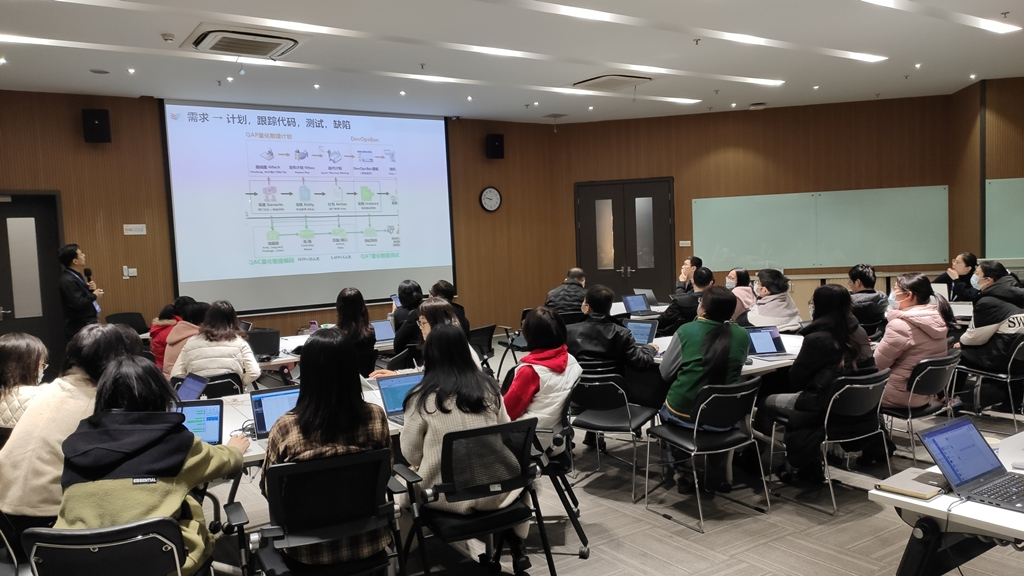
\includegraphics[width=10cm]{000.jpg}

图9-4

\hypertarget{ux540eux8bb0}{%
\section{后记}\label{ux540eux8bb0}}

\hypertarget{ux6708-ux4e0eux73b0ux573aux54a8ux8be2ux987eux95eeux5bf9ux8bdd}{%
\subsubsection{12月
与现场咨询顾问对话}\label{ux6708-ux4e0eux73b0ux573aux54a8ux8be2ux987eux95eeux5bf9ux8bdd}}

咨询顾问：``客户（A公司）现在人手紧张，都忙于交付项目，可能希望先简单快速完成级别评估，后面才慢慢实行真正的改善。''\\
评估师：``建议继续坚持做好改善才可以。因为有评估才能有效驱动团队抽出时间来做改善，很多领导都会说请放心，我们先快速拿证，后面才真正做改善，但我从未见过企业做到。你觉得我发你的过程改进资料有实用价值吗?''\\
咨询顾问：``你建议的各种方法论，如果给一些较成熟的软件开发公司是合适的。只是现在各团队，实在太忙，有心无力。''\\
评估师：``所以问题核心是要腾出时间，这也是要有计划的目的。我们自己要相信他们员工和管理层是具备所需的能力。从首次见面看得出高层万总很有魄力，做事有决心，相信他有能力解决中层、部门经理不投入、不配合这个关键问题。其他需要解决的问题都会水到渠成。''

\begin{description}
\tightlist
\item[]
= = = =
\end{description}

咨询顾问与COO万总开会汇报，并了解到为什么项目经理王工第一位提交改进计划，原来他的领导一直关注CMMI的进展。万总决定立马内部开紧急会议并敦促其他3位领导，要求每个小组必须按照要求针对缺陷与返工每迭代做质量改进。\\

回顾过去6个多月，虽然启动了，也做了培训、定期开会，但一直没有任何实际的改进。所以必须具备关键成功因素，如：领导的关注和支持、团队有时间和能力推进、制定计划、安排人手、按计划执行、一轮一轮逐步改善，就是这么简单。但确实要做到并不容易。

\hypertarget{ux9644ux4ef6}{%
\section{附件}\label{ux9644ux4ef6}}

\hypertarget{ux7761ux8863ux5de5ux5382ux5b9eux9a8c-harwood-manufacturing}{%
\subsection{睡衣工厂实验 Harwood
Manufacturing}\label{ux7761ux8863ux5de5ux5382ux5b9eux9a8c-harwood-manufacturing}}

二战后，在维京尼亚州有一家专门做睡衣的工厂Harwood。\\
难题：\\
要按不同的季节需求，做不同款式的睡衣，但往往有些女工习惯了某种工作方式，效率很高，但是要她改变工作方式，就接受不了，很难转换。

实验------比较3种变更方式：\\
\#按传统方式，依赖工程师去设计每一轮的变更。团队只需要按设计去做

\begin{enumerate}
\tightlist
\item
  每个团队有代表与管理层去讨论如何变更，然后执行
\item
  自己去策划自己的变更，也提建议。也安排那些女工每周跟那些生产率高和低的女工一起讨论不同方式的优劣，自己讨论怎么改变
\end{enumerate}

实验结果\\
*第一组按传统强制要求她们改变，花了3个月的时间，并引起很多不满，效果也不理想：生产率降低了20\%，也发现10名女工里面有一位后面就辞职不做了

\begin{itemize}
\tightlist
\item
  第二组效果中等，需要大概2周才恢复到本来的水平
\item
  第三组发现2天后就已经返回本来变更前的生产力水平，后面慢慢的上升提高到40\%。例如某实验组就把本来一天45件，5天后提升到87件------一个本来无法想象的数字，后面甚至提到90件，超越那些工业工程师本来的目标\\
\end{itemize}

\hypertarget{ux7caeux98dfux5206ux914dux5b9eux9a8c}{%
\subsection{粮食分配实验}\label{ux7caeux98dfux5206ux914dux5b9eux9a8c}}

二战时，美国虽然不是战区，也需要控制粮食供应。政府面对的难题：

\begin{itemize}
\tightlist
\item
  怎么让那些家庭的消费习惯，满足战时的食物供应\\
\end{itemize}

比如当时有些食物是要分配的，如何让家庭多吃一些供应充足的食物，避开紧缺的食物。他们实验发现，首先要知道整个过程是家庭里哪个人做这一块的决定。\\
研究分析发现，绝大部分的家庭都是由家庭主妇决定购买什么、储存什么、怎么做菜，丈夫没有太多的意见，通常是由妻子决定。

\textbf{实验设计}：

\begin{itemize}
\tightlist
\item
  把家庭主妇分成2组:
\end{itemize}

\begin{enumerate}
\tightlist
\item
  专家跟一组家庭主妇宣扬某种食物营养丰富，对家人的身体都会有好处
\item
  另一组家庭主妇没有专家指导，只是给她一些营养的数据，邀请主妇分成小组自己讨论决定怎么去做\\
\end{enumerate}

\textbf{结果}：实验发现第一种方法没有效果，第二种效果却很好。

\hypertarget{ux4e92ux52a8ux5de5ux4f5cux574aworkshop}{%
\subsection{互动工作坊(workshop)}\label{ux4e92ux52a8ux5de5ux4f5cux574aworkshop}}

\hypertarget{ux539fux5219}{%
\subsubsection{原则}\label{ux539fux5219}}

\begin{itemize}
\tightlist
\item
  高层的支持(Top Level Buy-in )：高层参与整个过程，也表示高层的重视。
\item
  从整系统入手(Improve Whole
  Systems)：要企业改变成功，仅仅抓一个小模块是没用的，要求岗位相关人员都参与，让所有人都看到整个相关系统。
\item
  破冰-让人了解需要改变(Unfreeze -- need for change)：
  因为是工作坊形式的互动讨论，经过2-3天可以让所有相关人都了解改变的前因后果，和参与决策
\item
  整体参与(Everybody solves problems)
  ：整个团队都参与到讨论中，包括高层。而不是传统的高层策划再向下推广，不然没有参与，就没有承担的心，提高学员对改进的承担(commitment).
\item
  自己动脑筋：主持人/领导不会直接告诉你答案，而是通过一些讨论和分享的方式，引导学员自己找出痛点，分析并找出解决方案；每组都可以天马行空地出主意，但也会面对来自不同等级人员和评委的残酷批评
\item
  做实验/试点/游戏 (Experiment/
  pilot)：把平常要半年到一年的改进项目压缩到3天，但关键的重点都一起讨论过。但也好像一次有奖游戏，激励团队的参与。
\end{itemize}

\hypertarget{ux7279ux70b9}{%
\subsubsection{特点}\label{ux7279ux70b9}}

\begin{itemize}
\tightlist
\item
  ``把所有的相关者凑在一起`Whole System'in the
  room''------所有相关人员都参与。例如：项目管理过程改进参与者不仅仅是项目经理，还有利益相关者，包括团队成员、供货商、客户代表、上下游、其他支持类部门等，可能都要参与
\end{itemize}

\begin{description}
\item[]
\begin{description}
\tightlist
\item[]
（目的：所有与系统相关的人都能对全局有概念，而不仅仅看到自己的部分）
\end{description}
\end{description}

\begin{itemize}
\tightlist
\item
  顾问/老师不直接给答案/方案，只是引导、帮助学员找出方向。
\item
  用分组竞赛形式提高成员参与的积极性
\item
  所有人都可以提出批评和意见，不仅仅是从上到下的决策/教育，接纳所有的思路和意见（像一个镜子）
\item
  分4-8组，8-10人一组，需要有一个大而光亮的会议室，方便小组互动，大白板和架子，各种颜色的水笔，墙壁可以贴上小组的白纸等
\item
  培训期间里都最好不受外界打优，例如每人都上交手机
\end{itemize}

%\href{文件:微信图片_20241101153835.jpg}{500px}

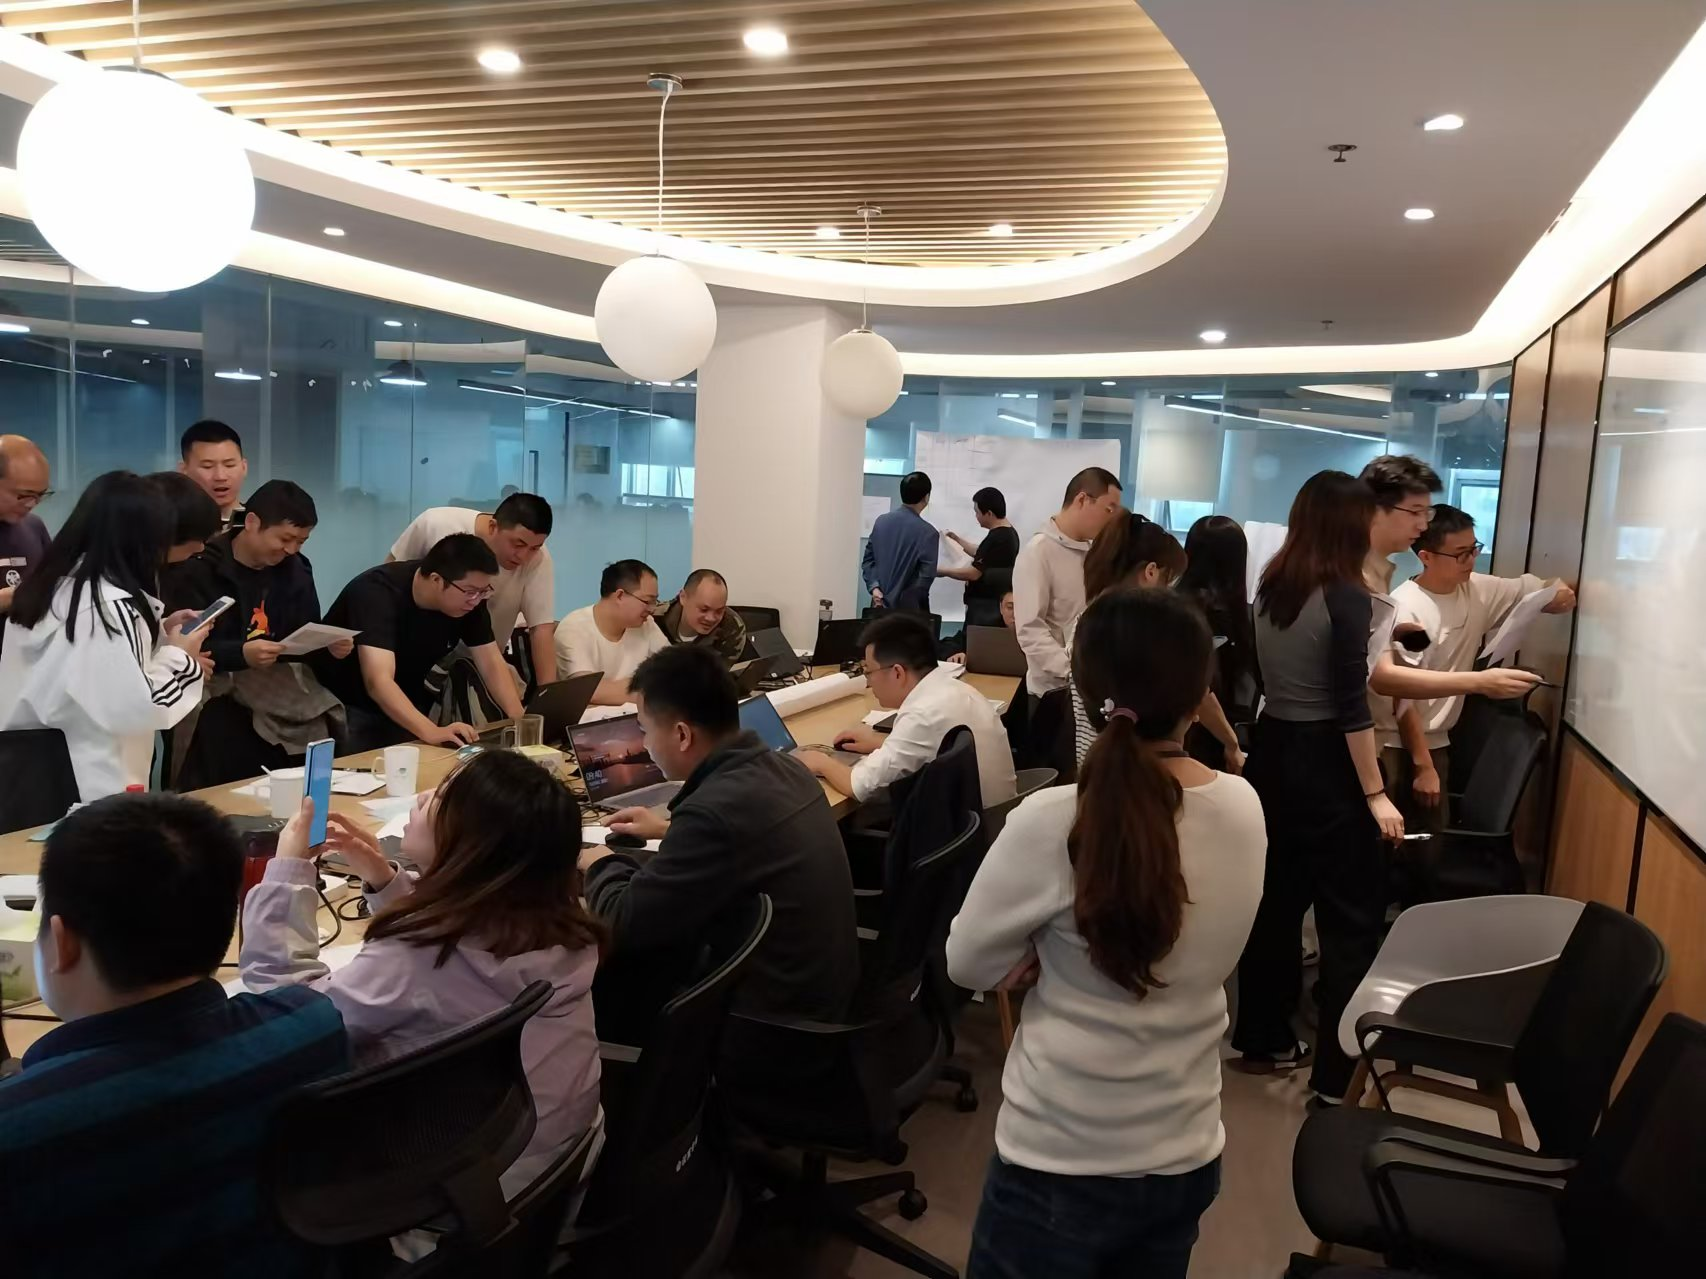
\includegraphics[width=3cm]{微信图片_20241101153835.jpg}

图9-5：每组有自己的``地盘''大家并行讨论

%\href{文件:13.1.jpg}{400px}

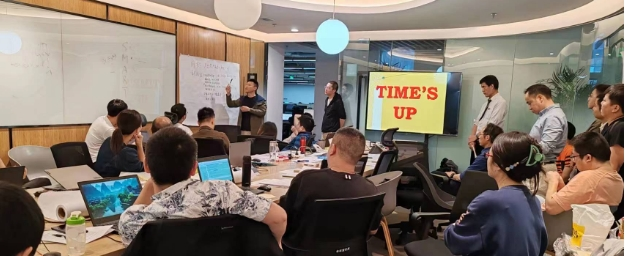
\includegraphics[width=3cm]{131.jpg}

图9-6：时间控制很重要，老师在屏幕投出余下分钟控制不超时

\hypertarget{ux6210ux529fux5173ux952eux8981ux7d20}{%
\subsubsection{成功关键要素}\label{ux6210ux529fux5173ux952eux8981ux7d20}}

1） 预先要有充分准备：

\begin{itemize}
\tightlist
\item
  建立行动委员会负责准备这次活动，活动的具体设计，在公司推进整个准备活动
\item
  主持人/协调人-对整个策划/准备/设计做辅导,
  现场活动包括（\textasciitilde{} 6 - 7 天）：

  \begin{itemize}
  \tightlist
  \item
    2天的策划会议
  \item
    1天详细设计
  \item
    2-3天工作坊 现场辅导 （包括事前的场地准备）
  \item
    1 天的事后回顾/跟进\\
  \end{itemize}
\end{itemize}

2）参会人员是否能够代表各相关角色？（能否包括整个系统 ，整体参与？）\\
3）高层是否全力支持和参与？

\hypertarget{ux53c2ux8003-references}{%
\section{参考 References}\label{ux53c2ux8003-references}}

\begin{enumerate}
\tightlist
\item
  Weisbord, M. , \emph{Future Search}
\item
  Hammer, M., Champy, J.\emph{Reengineering the Corporation}
\end{enumerate}


